\chapter{Growth shrink models}

\resp{Mezquita, Tomás}


\section{Theoretical background}

Growth models are very crucial in the study of complex networks. These models start from an initial network and incrementally add nodes and edges, leading to changes in the network topology and connectivity. One of the most important growth model it's the Barabasi-Albert preferential attachment model. In this model, new nodes tend to attach to well-connected nodes, resulting in a "rich-get-richer effect" that amplifies the connectivity of high-degree nodes while completing the network with new less connected nodes. This mechanism leads to interesting properties like a scale-free topology, which can be used to study real-life networks exhibiting such characteristics.

In contrast, shrink models involve removing nodes and their connections. These removals will affect the network by lowering its connectivity. The two principal shrink models involve the random removal of nodes and its connections or the targeted removal of nodes, for instance, removing the higher degree nodes. 

The objective of this project is to examine how growth and shrink models affect the network topology, connectivity and the emergence of scale-free properties while varying the parameters of the model.

 
\section{Results}



In order to achieve our objectives and obtain meaningful results, we will implement the following computational structure: 
\begin{enumerate}
    \item \textbf{Initialize the network}:  We start with a basic graph. For simplicity, we use an Erdos-Renyi network with a specified number of initial nodes and a connection probability.
    \item \textbf{Growth Phase}: We then add nodes to the network. Each new node connects to existing nodes based on their degree, following the Barabasi-Albert preferential attachment model.
    \item \textbf{Shrink Phase}: Finally, we perform the shrink phase by randomly removing nodes and their connections from the network.
\end{enumerate}

Throughout these phases, representative magnitudes of the network have been computed in each step, to see the evolution of these magnitudes as the network changes.  

The set of parameters that we are going to work with are: number of initial nodes, connection probability, number of grow and shrink steps, and edges added per step in the grow phase (m).

As the space is reduced we have picked six representative cases or set of parameters to visualize the evolution of the network. Starting from small and large networks we have:

\begin{itemize}
    \item Sparse initial network with low edge addition (blue in the graph)
    \item Dense initial network with low edge addition (red in the graph).
    \item Dense initial network with high edge addition (green in the graph).
\end{itemize}






\begin{figure}[h!]
    \centering
    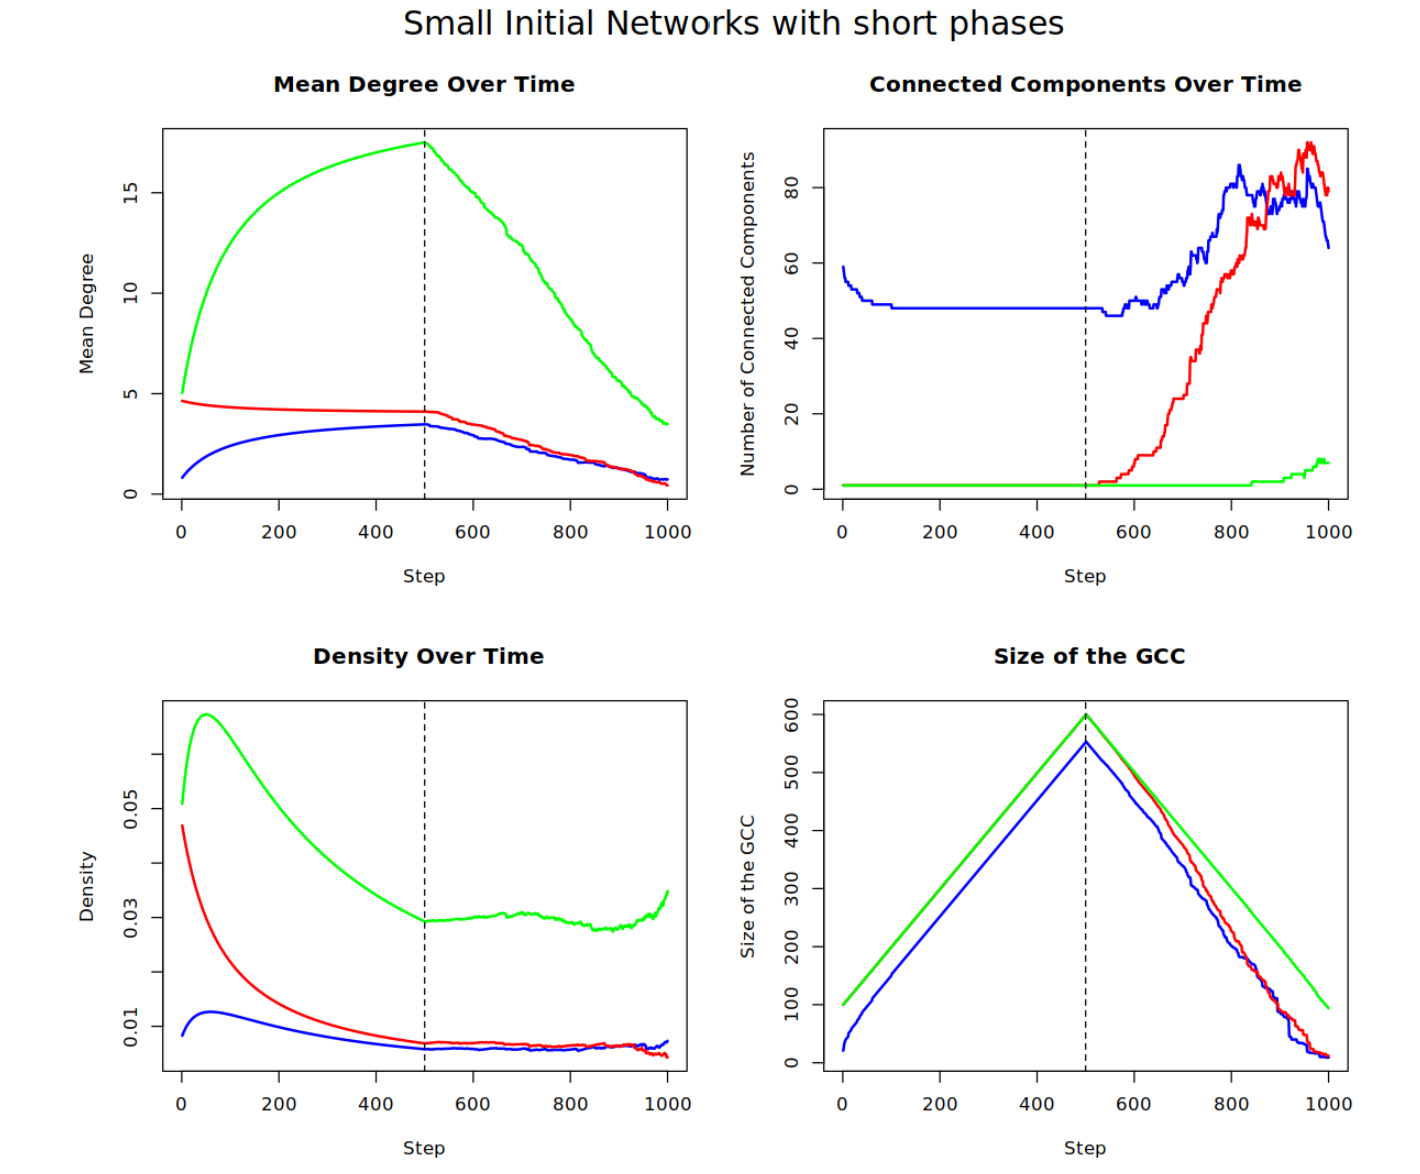
\includegraphics[width=0.49\textwidth]{images/magnitudes_small_ER.png}
    \hfill
    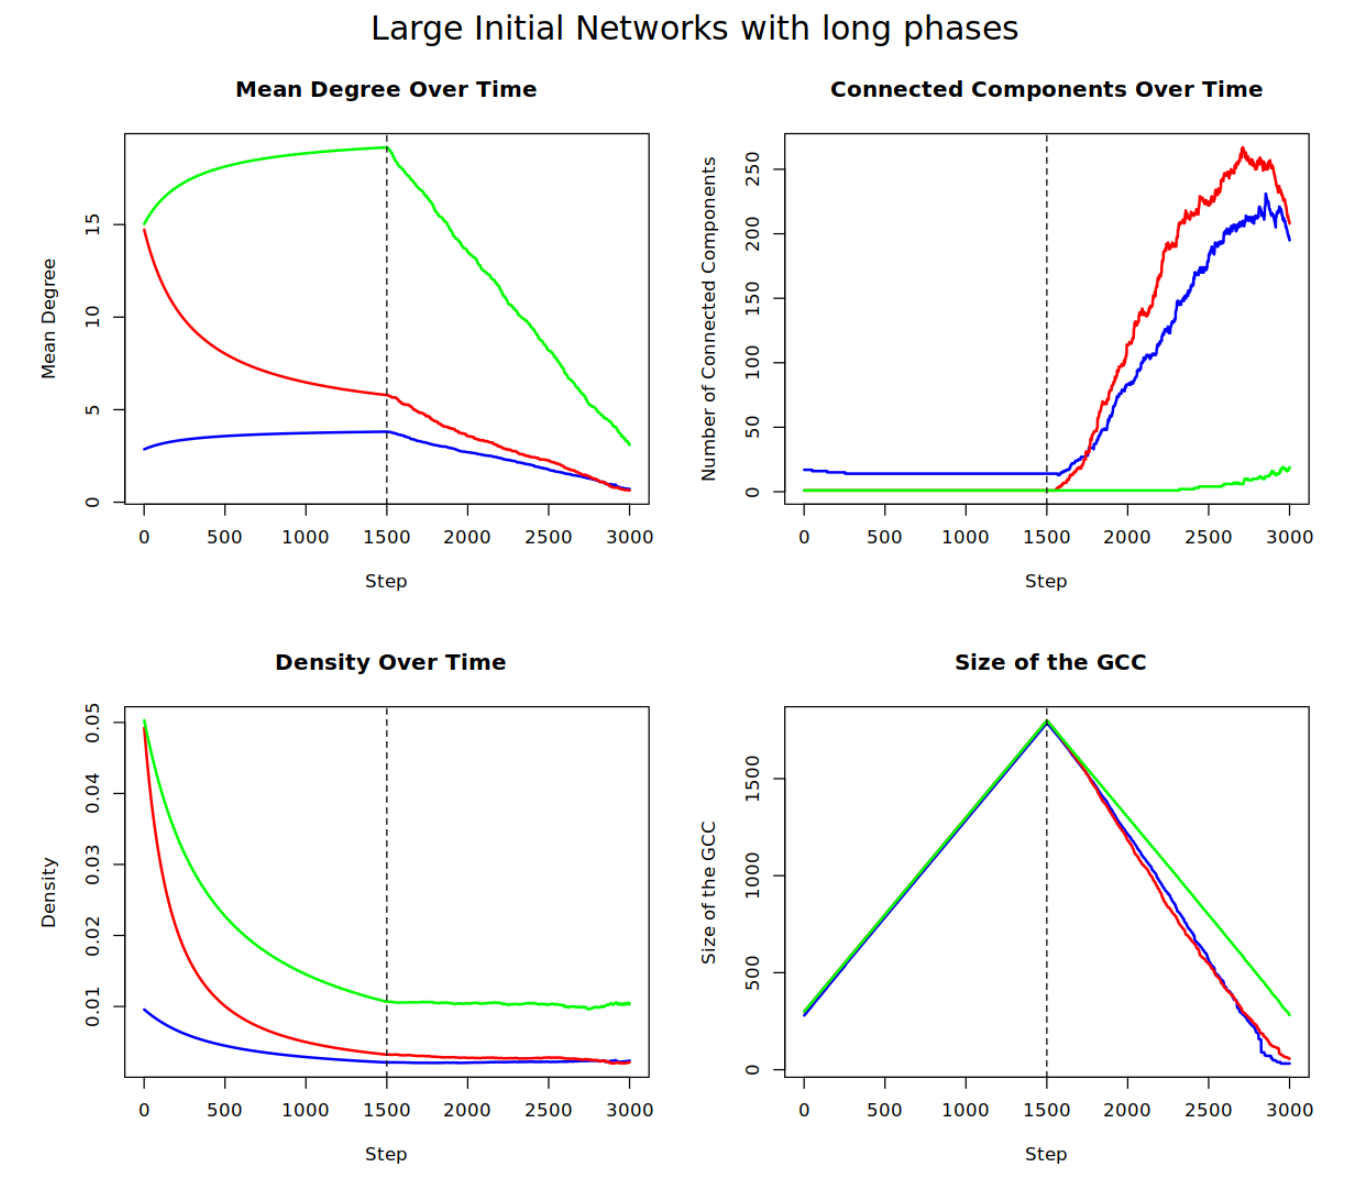
\includegraphics[width=0.49\textwidth]{images/magnitudes_large_ER.png}
\end{figure}
\begin{itemize}
    \item \textbf{Mean degree}: during the growth phase, the mean degree increases if the network is sparse and the edges added per step (m) are low. For denser networks, if m is insufficient, the mean degree may decrease as it already starts from a high mean degree. The mean degree tends to converge to \( \langle k \rangle = 2m \) as predicted. In the shrink phase, the mean degree decreases linearly, with randomness causing either abrupt or gradual decreases depending on node connectivity.
    \item \textbf{Connected components and size of GCC}: In the growth phase, if m is high relative to the initial network density, the density initially increases, reaching a peak before decreasing as the network size grows. For larger networks, density directly decreases. During the shrink phase, density remains roughly constant as edges are removed along with nodes.
    \item \textbf{Density} : In the growth phase, if m is high relative to the initial network density, the density initially increases, reaching a peak before decreasing as the network size grows. For larger networks, density directly decreases. During the shrink phase, density remains roughly constant as edges are removed along with nodes.

    
\end{itemize}

Other magnitudes, such as clustering coefficient and average path length, were computed, but are not showed as they show less variability. The clustering coefficient remains low, while the average path length tends to increase during the shrink phase.. 

The study of the degree distribution in the preferential attachment model its vital because it results in a power law distribution which help us understand the scale free networks.
We are going to see also how the shrink phase affect the degree distribution. 

\textbf{Degree distribution}

If the preferential attachment grow phase, degree distribution often follows a power law, that have the following structure $P(k)=k^{-\gamma}$. Using R programming I can obtain the degree distribution and visualize it, and also a power law fit which will give us the coefficient $\gamma$ and the R-squared to measure the quality of the fit. I have chosen an arbitrary network of 100 initial nodes and ER probability 0.05, 1000 grow steps, 500 shrink steps and 5 edges per growth step, and computed its distribution and fit at the initial graph, after the growth phase, and after the shrink phase. This are the results for an arbitrary network of:

\begin{figure}[h!]
    \centering
    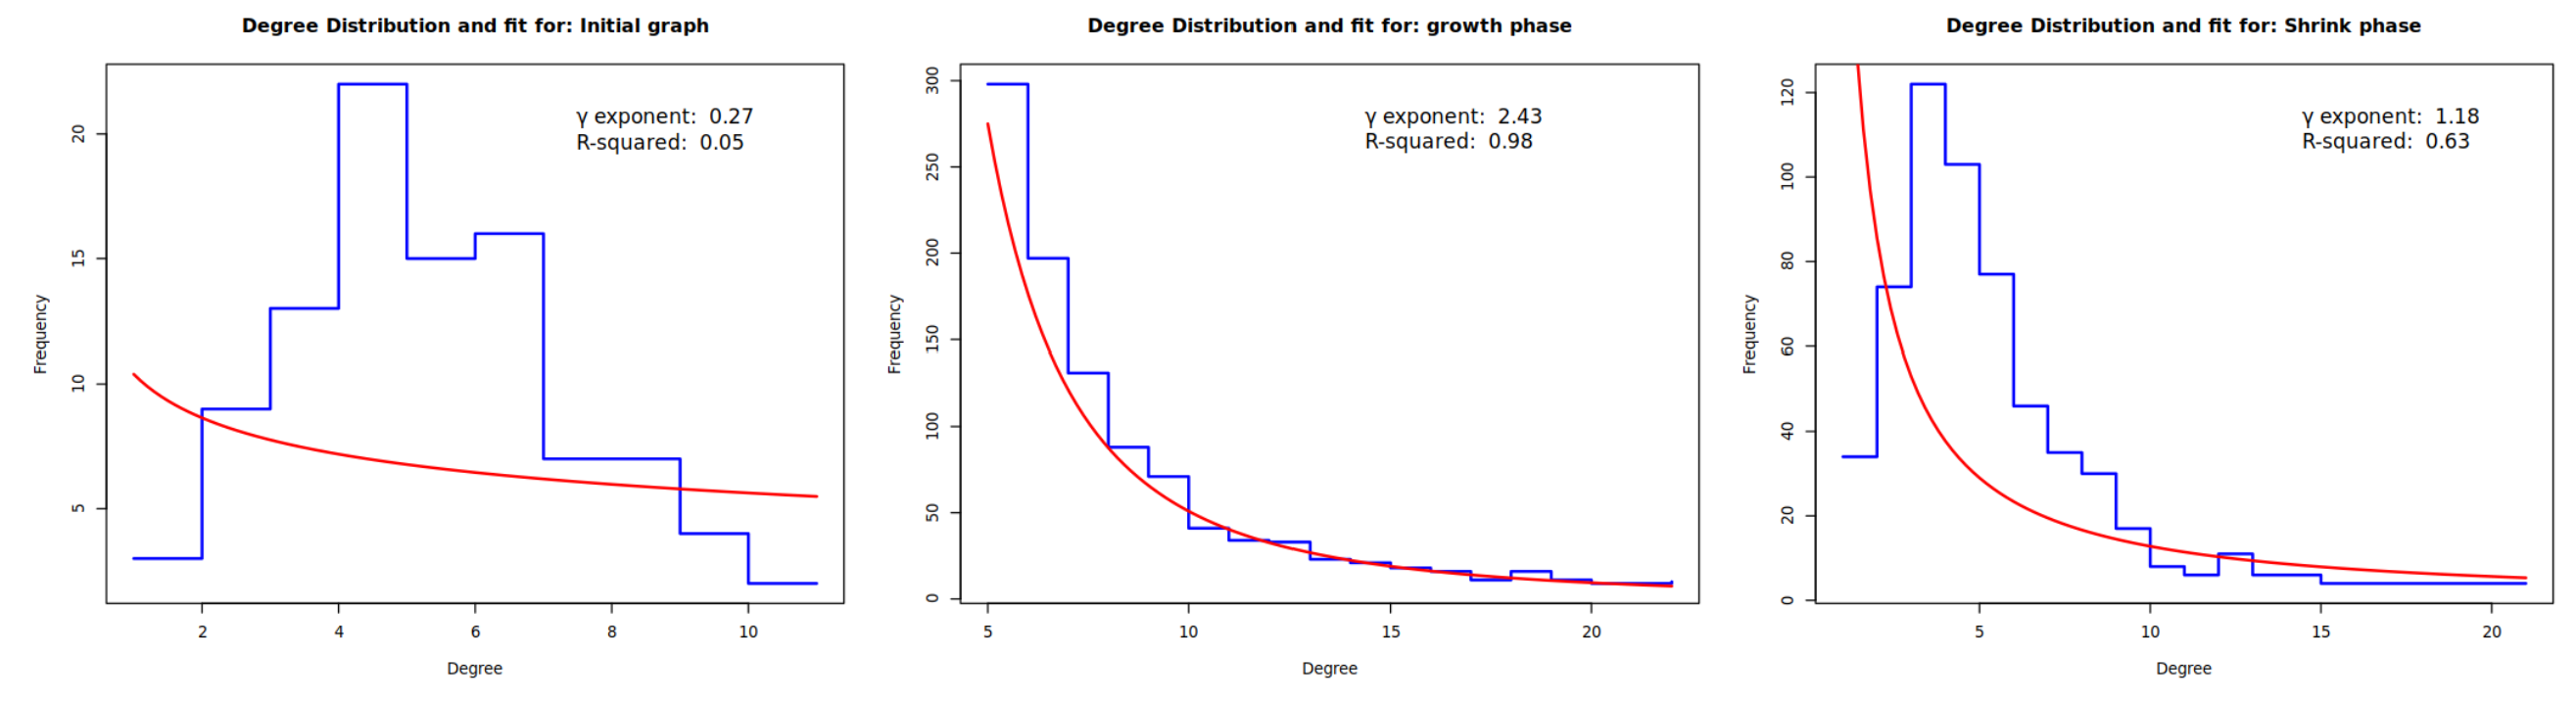
\includegraphics[width=1\textwidth]{images/degree_distr_pref.png}
\end{figure}

For the initial Erdos Renyi graph, where edges are placed randomly should follow a Poisson distribution centered around $<k>=Np=5$, as observed in the results. Therefore, the distribution doesn't fit to a power law.

As commented previously, during preferential attachment growth phase the power law/scale free nature starts to emerge. As shown in the middle graph, the degree distribution fits a power law, the value of R-squared close to 1 gives us proof that the fit is good. Also notice that all the nodes have degree larger than 5, which is consistent with the number of edges added per step. The $\gamma$ coefficient is 2.43, for pure Barabasi-Albert the expected coefficient is 3, but in general for scale free networks is $2<\gamma<3$ ~\cite{dedomeniconotes}, which aligns with our results.

After the shrink phase, the degree distribution deviates from the power law as nodes are removed randomly causing the emergence of a Poisson distribution for lower degree nodes.

Due to the limited space I couldn't explore new directions like trying for different initial networks, and different grow and shrink models, but I think they would be interesting to study in a more requiring project.

The study of the phenomena of grow shrink networks can help us understand some of the most important real life networks as networks are rarely static and tend to grow or shrink over time. Some examples of these networks are the world wide web, social networks, biological networks on species... 








